%
\section{Laundry data base library}

Mostly of the project subtasks decided to use one programming language to make easy work together. Sometimes different languages can be difficult connect and work together. That is why decided to use one object oriented language – C\#. As we know C\# is a new generation language which provides a lot of advance features like garbage collector and more others. This kind of language makes easier developer write programs, because here do not need take care about low level features like memory allocation or lost pointer. So this kind of language can decrease development process and increase code efficiency. 
Our case design was to store and provide data about the elders. All data were stored in MySQL data base. So many of subtask would like to use it and that is why were decided to create general library for any to use. Main design requirement is to create general library which has features:  reliable, easy maintain, simple to use, and easy update.

\subsection{Design phase}

To keep above mentioned requirement and features, decided to create a DLL (dynamic link library) which can be executable and contain inside code, data, and resources. Our design library inside have two classes:

\begin{itemize}
	\item MySQLConnection – data base connector which responsible for connection to data base and send/receive queries.
	\item Functions – general library for laundry data base.
\end{itemize}

\begin{figure}[h]
	\centering
		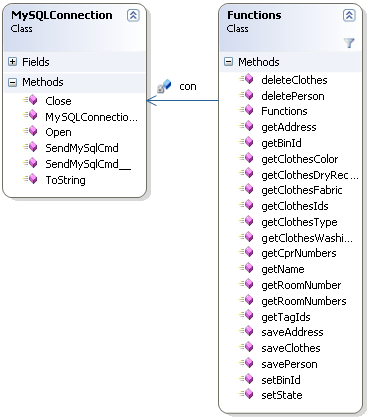
\includegraphics{classLibrary}
	\caption{Class library of the data base connection}
	\label{fig:planning}
\end{figure}

\subsection{Implementation}

Software development was related to unified process (UP) – iterative incremental process.  Iterative incremental process model [5] was used during the implementation.  
Let us explain everything in more detail. Project were created using class Library in Microsoft Visual C\# .NET 3.5. To have data base connection were included MySQL Connector Net 1.0.10 into references. To use created library we need include it into new project (Console or Win or else) and start our library. For example we insert our library into console project, so connection to data base is like shown in the figure 6.1. After successful connection we can use class functions and manage laundry data base. \\ Numbers explain data base connection parameters: 

\begin{enumerate}
	\item IP address or domain
	\item Data base name
	\item User Id
	\item Port number
	\item Password
\end{enumerate}

\begin{figure}[h]
	\centering
		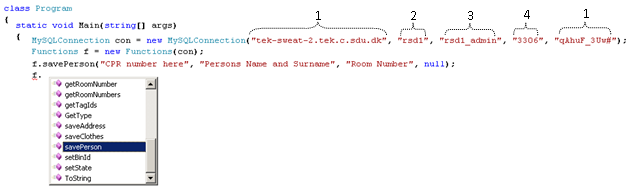
\includegraphics{connectionToData}
	\caption{Connection to data base server and save new person}
	\label{fig:planning}
\end{figure}

Class functions uses created instance of MySQLConnection library. And throw the variable f can be connected to all created methods. At the figure 6.2 shows an example of creation new person. As we can see there used methods send queries to data base. New CPR inserted into table person by query: “INSERT INTO Person (CPR) Values (‘1234567890’)”.


\begin{figure}[h]
	\centering
		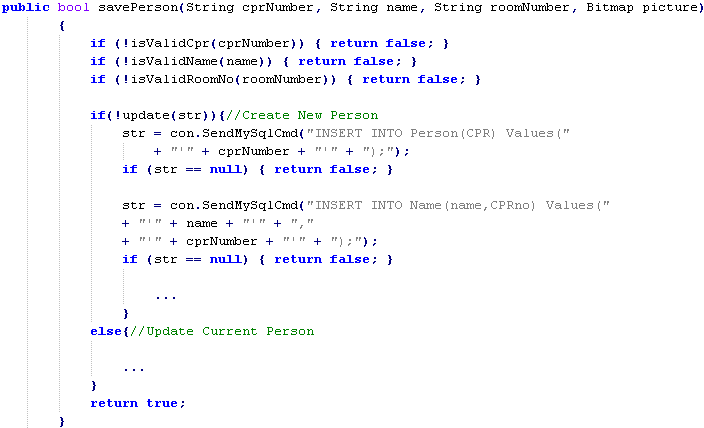
\includegraphics{exampleSavePerson}
	\caption{Example of save person method}
	\label{fig:planning}
\end{figure}

\subsection{Future work}